\documentclass[11pt]{article}
\usepackage{fancyhdr}
\usepackage[table]{xcolor}
\usepackage[margin=1in]{geometry}
\usepackage{caption}
\usepackage{hyperref}
\usepackage{graphicx}
\usepackage{float}


% Set header and footer
\pagestyle{fancy}
\fancyhf{}
\fancyhead[L]{USC Facilities: Rain Barrel Water Pump System} % Team name in the header
\fancyfoot[C]{\thepage} % Page number in the footer

\begin{document}

\title{
    \vspace{2in}
    \textbf{EMCH427-002} \\[1ex]
    \textbf{Needs Report} \\[1ex]
    \textbf{Sponsor: USC Facilities} \\[1ex]
    \vspace{2in}
}

\author{
    \textbf{Team Members:} \\[2ex]
    Tanner Harmon -- Worked on stakeholders and product mission \\[1ex]
    Presston McConnell -- Worked on methodology \\[1ex]
    William Wenzel -- Worked on prioritization and identification of needs \\[1ex]
    Jacob Vaught -- Worked on prioritization and identification of needs \\[2ex]
    \textbf{Note:} All team members contributed to the appendix.
}

\date{}

\maketitle
\thispagestyle{fancy} % Ensures header and footer are applied to cover page

\newpage

\section{Introduction to Project and Stakeholders}

This report identifies and prioritizes the needs of stakeholders in designing a sustainable water management system for the Green Quad Garden at USC, aiming to optimize water transfer, promote environmental stewardship, and encourage sustainable practices.

\subsection{Who: Office of Sustainability at USC}
The client, the Office of Sustainability in collaboration with the Carolina Sustainable Garden initiative, ensures the system aligns with USC's sustainability goals while addressing the garden’s operational needs.

\subsection{What: Sustainable Water Management System}
The project aims to create a user-friendly system to transfer rainwater from a 1,000-gallon tank to the garden, reducing manual labor, ensuring easy operation, and minimizing environmental impact while integrating into existing infrastructure.


\subsection{Stakeholders}
\subsubsection{Primary Stakeholders:}
\begin{itemize}
    \item Green Quad Residents: As daily users, residents maintain the garden and will benefit from a system that simplifies upkeep, making the space more enjoyable and educational.
    \item Garden Volunteers: This group, including students, faculty, and staff, seeks an efficient system to reduce watering efforts, allowing more focus on community activities.
    \item Office of Sustainability: The sponsor aims to promote sustainable practices, water conservation, and eco-friendly materials, using the project as a campus sustainability model.
\end{itemize}

\subsubsection{Secondary Stakeholders:}
\begin{itemize}
    \item Students and Faculty Using the Walkway: They value a seamless system that integrates into the garden without disrupting pedestrian traffic or visual appeal.
    \item University Visitors: Visitors, including prospective students, see the garden as a symbol of USC’s sustainability commitment, enhanced by a state-of-the-art system.
\end{itemize}

\subsubsection{Tertiary Stakeholders:}
\begin{itemize}
    \item USC Facilities Management: Responsible for long-term maintenance, they require a durable, low-maintenance solution.
    \item Campus Administration: Interested in sustainable projects that boost the university’s reputation and align with strategic goals.
\end{itemize}
\newpage
\section{Methodology}

\subsection{Data Collection Methods}
Various data collection methods were used to ensure a thorough assessment of the proposed water management system.

\subsubsection{Site Visit}
\begin{itemize}
    \item Site visit conducted on September 20th at 10 AM at the Green Quad garden (1216 Wheat Street, Columbia, SC).
    \item Observations included the current manual watering process and the time required.
    \item Inspections of the garden layout, rainwater tank placement, and surrounding infrastructure were conducted to assess system integration.
    \item Photographs documenting current conditions were taken and referenced in the Appendix (Figures 1-10).
\end{itemize}

\subsubsection{Interviews and Meetings}
\begin{itemize}
    \item Key meetings held with Donita Harris and Larry Cook from the Office of Sustainability.
    \item 30-minute Q\&A session to discuss client needs and expectations.
    \item Followed by a 20-minute on-site inspection to identify challenges and explore opportunities for the new system.
\end{itemize}

\subsubsection{Photographic Documentation}
\begin{itemize}
    \item Photographs were taken during the site visit to further analyze the garden and tank setup.
    \item Visual documentation provided in the Appendix, including close-ups of key equipment.
\end{itemize}

\subsubsection{Internet Research}
\begin{itemize}
    \item Additional data gathered through internet research on the Green Quad garden’s role within the university.
    \item Research focused on understanding the sustainability goals of the Office of Sustainability.
\end{itemize}

\subsection{Communications}
\begin{itemize}
    \item Team maintained communications with key stakeholders.
    \item Emails and meetings scheduled with Donita Harris (johnstdb@mailbox.sc.edu) and Larry Cook (lcook@mailbox.sc.edu) to gather further insights on system requirements and design expectations.
\end{itemize}


\newpage
\section{Interpretation of Needs}

\subsection{Overall Observations}

From the site visit and data collection, several key observations were made regarding the current watering system at the Green Quad Garden:

\begin{itemize}
    \item \textbf{Manual Watering Process:} The existing manual method of transferring water using 2-gallon cans is labor-intensive and time-consuming. Volunteers and residents perform this task frequently, highlighting the need for a more efficient system.
    
    \item \textbf{Garden Layout and Tank Placement:} The rainwater tank is located on a loading dock above the garden, which creates elevation challenges, affecting water pressure and the consistency of water flow throughout the garden.
    
    \item \textbf{User Involvement:} Various users, including students, faculty, and community volunteers, engage in garden maintenance. Therefore, the watering system must be accessible to individuals with different physical abilities and knowledge levels.
    
    \item \textbf{Water Conservation Concerns:} Efficient water use is a priority. The current system lacks monitoring and control capabilities, leading to potential water wastage during the manual watering process.
    
    \item \textbf{Sustainability Goals:} The new system must align with USC’s broader sustainability objectives, promoting eco-friendly practices and maximizing the efficient use of water resources.
\end{itemize}



\newpage
\section{Derivation of Needs}

\subsection{Operational Efficiency Needs}

\subsubsection{Time-efficient water transfer}
The system should minimize the time required to move water from the tank to the garden, replacing the manual 2-gallon cans.

\subsubsection{Minimal manual intervention}
The system must operate with little hands-on effort, allowing one person to manage the watering process easily.

\subsubsection{Efficient water distribution}
Water must be delivered evenly across the entire garden, avoiding under- or over-watering.

\subsubsection{Continuous operation}
The system should run without frequent start-stop interruptions to improve efficiency.

\subsubsection{Minimal water wastage}
Water wastage should be minimized, especially when using collected rainwater.

\subsubsection{Consistent water output}
Water flow and pressure must remain steady throughout the watering session.

\subsubsection{Flexible watering schedules}
The system must adapt easily to varied watering schedules based on plant and weather needs.

\subsubsection{Scalability for expansion}
The system should accommodate garden expansion or additional water tanks without major modifications.

\subsubsection{Easy monitoring of water usage}
The system must allow easy tracking of water usage and distribution.

\subsubsection{Adaptable to water demand}
The system should adjust its output based on varying water demand or supply conditions.

\subsubsection{Peak demand functionality}
The system should handle large water volumes efficiently during peak demand periods.

\subsubsection{Quick activation and deactivation}
It should be easy to start and stop the system when needed.

\subsubsection{Adaptability to garden layout changes}
The system must easily adjust to changes in the garden layout or design.

\subsubsection{Effective with varying water volumes}
The system must handle both high and low water volumes reliably.

\subsubsection{Minimized physical effort}
Operating the system should require minimal physical strain for users.

\subsubsection{Easy setup for different garden zones}
The system should be easy to configure for different garden zones with varying water needs.

\subsubsection{Adjustable water flow for plant needs}
Water flow must be adjustable to suit different plant requirements.

\subsubsection{Rapid deployment or removal}
The system should be easy to set up or dismantle as needed.

\subsubsection{Quick troubleshooting}
The system should allow for quick identification and correction of operational issues.

\subsubsection{Seamless recovery after interruptions}
The system should resume normal operation quickly after any interruptions.

\newpage
\subsection{Pressure and Flow Needs}

\subsubsection{Sufficient water pressure}
The system must provide adequate pressure for effective water delivery across the garden.

\subsubsection{Consistent pressure with elevation changes}
Water pressure must remain steady, even with elevation differences in the garden.

\subsubsection{Prevention of pressure drops}
The system should prevent significant pressure drops during operation.

\subsubsection{Adjustable water pressure}
Water pressure must be adjustable for different irrigation applications.

\subsubsection{User feedback on pressure}
Users should be informed about current pressure levels for proper system operation.

\subsubsection{Pressure maintenance over long distances}
The system must maintain adequate pressure even when water is delivered over long distances.

\subsubsection{Even water distribution}
Water should be distributed evenly across the entire garden.

\subsubsection{Prevention of pressure surges}
The system should avoid pressure surges that could damage components.

\subsubsection{Functionality under varying pressure}
The system should operate efficiently under both high and low pressure conditions.

\subsubsection{Adequate flow rate for irrigation}
The system should provide the necessary flow rate for different irrigation methods.

\subsubsection{Detection and correction of flow issues}
Flow problems should be easy to detect and correct.

\subsubsection{Flow maintenance in low-pressure conditions}
The system should maintain water flow even under low-pressure scenarios.

\subsubsection{Consistency with fluctuating water levels}
Water flow must remain consistent even as tank levels fluctuate.

\subsubsection{Consistent water delivery across garden}
Water should be delivered evenly, regardless of garden layout or distance from the tank.

\subsubsection{Gradual pressure changes}
Pressure changes should be smooth to avoid system damage.
\subsubsection{Easy verification of flow performance}
Users should easily verify if the system is delivering the expected flow rate.

\subsubsection{Minimal disruption during adjustments}
Adjustments to pressure or zones should not cause significant disruption to water flow.

\subsubsection{Operation at high and low flow rates}
The system must function efficiently with both high and low flow rates, depending on the watering needs.

\subsubsection{Consistent flow under varying conditions}
The system should maintain a steady flow even with external factors like weather or temperature fluctuations.

\subsubsection{Optimal flow for irrigation methods}
Each irrigation method must receive the optimal flow rate for efficient water delivery.

\newpage
\subsection{Usability Needs}

\subsubsection{Easy operation for non-technical users}
The system should have a simple interface that allows non-technical users to operate it without specialized training.

\subsubsection{Clear instructions for use}
The system should provide clear, step-by-step instructions to guide users through setup, operation, and maintenance.

\subsubsection{Minimal training required}
The system should be intuitive to set up and use, requiring minimal training or prior experience.

\subsubsection{Accessible to users with different physical abilities}
The system should be designed to accommodate users of varying physical capabilities, ensuring ease of use for all.

\subsubsection{Operational feedback}
The system should provide clear visual or audible feedback on its operational status to inform users.

\subsubsection{Easy start-stop functionality}
The system should allow users to start, stop, and adjust settings quickly and easily.

\subsubsection{Quick user familiarization}
The system should be easy to learn, ensuring that users become familiar with its operation quickly.

\subsubsection{Configuration for different watering needs}
The system should allow users to configure it easily for different garden zones and plant types.

\subsubsection{Visible indicators for key parameters}
Key operational parameters, like water pressure and flow rate, should be clearly displayed for easy monitoring.

\subsubsection{Minimized operational steps}
The system should require as few steps as possible for operation, reducing complexity.

\subsubsection{Clear operational guidelines}
Any provided guidelines should be clear and easy to understand, ensuring correct operation.

\subsubsection{Usable in various lighting conditions}
The system should be designed to be operable in both daylight and low-light conditions.

\subsubsection{Clear labeling of components}
All user-accessible components, such as valves or switches, should be clearly labeled.

\subsubsection{Easy performance monitoring}
The system should allow users to easily check performance metrics, such as water usage or settings.

\subsubsection{Low physical exertion required}
Operating the system should not require significant physical effort, making it accessible to all users.

\subsubsection{Easy reset or reconfiguration}
The system should be easy to reset or reconfigure when necessary, without complex steps.

\subsubsection{Quick emergency shutdown}
The system should have an easy-to-use emergency shutdown feature in case of malfunction.

\subsubsection{No need for specialized tools}
The system should be operable and maintainable without the need for specialized tools.

\subsubsection{Comfortable for extended use}
The system should be comfortable to use for extended periods without causing fatigue.

\subsubsection{Minimizes user errors}
The system should be designed to prevent confusion or errors during operation.

\newpage
\subsection{Maintenance Needs}

\subsubsection{Minimal maintenance required}
The system should require minimal maintenance for reliable operation.

\subsubsection{Easy access to maintenance components}
Parts needing regular attention, like filters or valves, should be easy to reach.

\subsubsection{Infrequent maintenance interventions}
The system should need maintenance only at long intervals to reduce downtime.

\subsubsection{Easy identification of components needing service}
Components requiring maintenance should be clearly marked or have indicators.

\subsubsection{Easy to clean and maintain}
The system should be straightforward to clean and maintain regularly.

\subsubsection{Maintenance alerts}
The system should provide visual or audible alerts when maintenance is required.

\subsubsection{Minimized component failure risk}
The system should be designed with high-quality materials to minimize the risk of component failure.

\subsubsection{Durable against wear and tear}
The system should withstand regular use without degrading quickly.

\subsubsection{Easy replacement of consumable parts}
Parts like filters should be easy to replace with simple instructions.

\subsubsection{Routine maintenance simplicity}
Routine maintenance tasks should be easy to complete without special tools.

\subsubsection{Functionality with minor wear}
The system should continue to work effectively even with minor wear or faults.

\subsubsection{Prevention of maintenance escalation}
The system should include features that prevent small issues from becoming major problems.

\subsubsection{Resistance to clogging}
The system should be designed to avoid clogging, particularly when using rainwater.

\subsubsection{No need for specialized tools}
Maintenance should be possible using basic tools.

\subsubsection{Durable in indoor and outdoor conditions}
The system should be resistant to environmental factors, such as weather exposure.

\subsubsection{Accessible maintenance log}
The system should maintain a clear log of all maintenance activities.

\subsubsection{Easy troubleshooting}
The system should provide simple troubleshooting for common issues.

\subsubsection{Simple drainage and storage}
The system should be easy to drain and store when not in use.

\subsubsection{Protection against external damage}
The system should have protection against potential damage from animals or vandalism.

\subsubsection{Adaptability to seasonal changes}
The system should be easy to prepare for different seasons, like winterization.

\newpage
\subsection{Environmental Impact Needs}

\subsubsection{Minimized environmental impact}
The system should be designed to minimize its negative effects on the local ecosystem.

\subsubsection{Sustainable and recyclable materials}
The system should prioritize the use of sustainable, recyclable materials to reduce waste.

\subsubsection{Energy efficiency}
The system should be energy-efficient and, where possible, utilize renewable energy sources.

\subsubsection{No contamination to water or soil}
The system should avoid introducing harmful substances into the water or soil.

\subsubsection{Reduced water wastage}
The system should be designed to deliver only the necessary water to avoid wastage.

\subsubsection{Alignment with sustainability goals}
The system should support the sustainability goals of the garden and project site.

\subsubsection{No disruption to local wildlife}
The system should not disturb local wildlife or their habitats.

\subsubsection{Compatibility with eco-friendly practices}
The system should work with existing sustainable practices, such as composting and organic gardening.

\subsubsection{Support for renewable resources}
The system should encourage the use of renewable resources like harvested rainwater.

\subsubsection{Minimized noise pollution}
The system should operate quietly, reducing noise pollution in the garden area.

\subsubsection{Seamless integration into infrastructure}
The system should fit into the existing environmental infrastructure without major modifications.

\subsubsection{Resistance to extreme weather}
The system should withstand harsh environmental conditions, like strong winds or heavy rain.

\subsubsection{Minimized carbon footprint}
The system should be designed to produce a minimal carbon footprint throughout its lifecycle.

\subsubsection{Conservation of natural resources}
The system should promote the efficient use of water and energy to conserve natural resources.

\subsubsection{Prevention of soil erosion}
The system should control water delivery to prevent soil erosion and protect plant health.

\subsubsection{Adaptability to changing regulations}
The system should be flexible enough to comply with evolving environmental regulations.

\subsubsection{No pollution to local water sources}
The system should prevent runoff or leaching that could pollute nearby water sources.

\subsubsection{Safe for plants and humans}
Materials used in the system should be non-toxic and safe for both plants and humans.

\subsubsection{Compatibility with rainwater harvesting}
The system should integrate seamlessly with rainwater harvesting practices.

\subsubsection{Long-lasting with minimal environmental impact}
The system should be durable, reducing the need for frequent replacements, and minimize its long-term environmental impact.

\newpage
\subsection{Cost and Budgetary Needs}

\subsubsection{Cost-effective implementation}
The system should be affordable to design and install within the given budget.

\subsubsection{Low operational costs}
The system should have minimal ongoing costs for operation, such as energy use and maintenance.

\subsubsection{Stay within budget}
The total cost of the system should not exceed the specified maximum budget.

\subsubsection{Balance cost and performance}
The system should prioritize cost-saving without sacrificing performance.

\subsubsection{Flexible budgeting}
The system should allow flexibility in allocating budget to different components if needed.

\subsubsection{Avoid high ongoing costs}
The system should avoid requiring expensive maintenance or consumables over time.

\subsubsection{Leverage existing resources}
The system should utilize existing infrastructure to minimize additional expenses.

\subsubsection{Durability and efficiency for value}
The system should provide good value through long-term durability and efficient performance.

\subsubsection{Minimize consumable costs}
The system should avoid requiring expensive consumable parts that need frequent replacement.

\subsubsection{Predictable maintenance and repair costs}
The system should have predictable costs for future maintenance and repairs.

\subsubsection{Operational savings}
The system should contribute to cost recovery through efficiency, reducing labor or water costs.

\subsubsection{Cost-benefit analysis}
The system should include a clear breakdown of expected costs and benefits.

\subsubsection{Support for future upgrades}
The system should allow for potential upgrades without significant additional costs.

\subsubsection{Designed with cost-effectiveness in mind}
Cost-effectiveness should be considered from the start of the design process.

\subsubsection{Scalability without significant cost increases}
The system should be scalable without adding substantial costs.

\subsubsection{Avoid unexpected costs}
All potential costs should be accounted for to prevent budget overruns.

\subsubsection{Use of durable components}
The system should use high-quality materials to reduce the frequency of replacements.

\subsubsection{Minimize financial risk}
The system should be designed to minimize financial risks, such as cost overruns or poor performance.

\subsubsection{Cost-efficient disposal or recycling}
The system should be easy and affordable to dispose of or recycle at the end of its lifecycle.

\subsubsection{Long-term financial sustainability}
The system should consider long-term costs, including upkeep and potential savings over time.

\newpage
\subsection{Safety and Compliance Needs}

\subsubsection{Compliance with safety standards}
The system should meet all relevant safety codes and regulations.

\subsubsection{Safe operation in various weather conditions}
The system should operate safely under diverse weather conditions, including rain, wind, and heat.

\subsubsection{Prevention of accidental misuse}
The system should have safeguards to prevent accidental or incorrect operation.

\subsubsection{No sharp edges or hazardous components}
User-accessible components should be free from sharp edges or hazards.

\subsubsection{No risks to pedestrians or garden users}
The system should not create hazards for people in the garden, such as tripping or slipping risks.

\subsubsection{Clear hazard labeling}
Components with potential risks should be clearly labeled with warnings.

\subsubsection{Prevention of water contamination}
The system should avoid contaminating water sources with harmful substances.

\subsubsection{Durable against accidental impacts}
The system should withstand minor impacts without compromising safety or functionality.

\subsubsection{Unobstructed emergency access}
The system should not block emergency exits or routes in the garden.

\subsubsection{Protection against tampering}
The system should include measures to prevent unauthorized access or tampering.

\subsubsection{Compliance with environmental regulations}
The system must comply with all local environmental regulations related to water use and disposal.

\subsubsection{No interference with infrastructure}
The system should not interfere with existing utilities or infrastructure.

\subsubsection{Prevention of tripping or slipping hazards}
The system should be installed to avoid creating any tripping or slipping hazards.

\subsubsection{Stable and secure setup}
The system should remain stable and secure, whether in use or not.

\subsubsection{No harmful emissions or pollutants}
The system should not release harmful emissions into the air, water, or soil.

\subsubsection{Clear safety instructions}
Users should receive clear and concise safety instructions for operation and maintenance.

\subsubsection{Minimized risk of fire or electrical hazards}
The system should be properly insulated and grounded to avoid electrical hazards or fires.

\subsubsection{Secure components}
All system components should be properly fastened to prevent loosening or detachment.

\subsubsection{Resistance to vandalism or accidental damage}
The system should be designed to withstand acts of vandalism or accidental damage.

\subsubsection{Emergency shutdown procedures}
The system should have clear, documented procedures for emergency shutdowns.

\newpage
\section{Prioritization of Needs}

\subsection{Process Explanation}
\begin{itemize}
    \item The prioritization process was conducted in three steps to systematically identify and rank the most critical needs for the water management system project.
    \item This structured approach ensured equal input from each team member.
    \item Needs that advanced to the next stage are highlighted in yellow.
\end{itemize}

\subsubsection{Customer Requirement Prioritization (Round 1)}
\begin{itemize}
    \item Each team member was given 140 points to distribute across all identified needs.
    \item Points were allocated based on the perceived importance of each need.
    \item The purpose of this round was to filter out lower-priority needs.
    \item The top 24 needs with the highest cumulative points advanced to Round 2 (Table 1).
\end{itemize}

\subsubsection{Critical to Quality (CTQ) Needs Ranking (Round 2)}
\begin{itemize}
    \item Each team member was allocated 24 points to distribute across the remaining 24 needs.
    \item This round aimed to further narrow down the list.
    \item The top 6 needs with the most points advanced to the final round (Table 2).
\end{itemize}

\subsubsection{Final Ranking (Round 3)}
\begin{itemize}
    \item Each team member ranked the top 6 needs by assigning 1 to 6 points, with 6 being the highest priority.
    \item The final ranking determined the priority order of the most critical needs (Table 3).
\end{itemize}


\newpage
\subsection{Affinity Diagrams}

\subsubsection{Table 1: Needs Prioritization}


\begin{table}[H]
\centering
\caption*{Table 1a: Operational efficiency needs.}
\label{table:1a}
\rowcolors{2}{lightgray}{}
\begin{tabular}{|p{10cm}|c|c|c|c|c|}
\hline
\textbf{Need} & \textbf{\#1} & \textbf{\#2} & \textbf{\#3} & \textbf{\#4} & \textbf{Sum} \\
\hline
1.1. The system should minimize the time required to transfer water from the tank to the garden. & 5 & 6 & 7 & 4 & \cellcolor{yellow}22 \\
1.2. The system must operate effectively with minimal manual intervention. & 0 & 1 & 0 & 0 & 1 \\
1.3. Water distribution should cover the entire garden area efficiently. & 4 & 4 & 2 & 5 & \cellcolor{yellow}15 \\
1.4. The system should be able to operate without frequent start-stop interruptions. & 0 & 0 & 0 & 1 & 1 \\
1.5. The system should ensure minimal water wastage during operation. & 3 & 1 & 0 & 2 & 6 \\
1.6. Water output should be consistent and reliable during the watering process. & 3 & 3 & 2 & 3 & \cellcolor{yellow}11 \\
1.7. The system should be flexible enough to handle varying watering schedules. & 0 & 0 & 4 & 1 & 5 \\
1.8. The system should be scalable to handle garden expansion or additional tanks. & 0 & 1 & 2 & 2 & 5 \\
1.9. The system should allow for easy monitoring of water usage and distribution. & 0 & 0 & 0 & 1 & 1 \\
1.10. The system should be able to adapt to water demand and supply conditions. & 0 & 0 & 0 & 0 & 0 \\
1.11. The system should maintain functionality during peak water demand periods. & 2 & 1 & 2 & 1 & 6 \\
1.12. The system should be easy to activate and deactivate when needed. & 3 & 2 & 5 & 2 & \cellcolor{yellow}12 \\
1.13. The system should be adaptable to changes in garden layout or design. & 0 & 0 & 0 & 0 & 0 \\
1.14. The system should be able to handle variable water volumes effectively. & 1 & 1 & 0 & 2 & 4 \\
1.15. The system should minimize the physical effort required to operate it. & 3 & 2 & 2 & 1 & \cellcolor{yellow}8 \\
1.16. The system should be easy to set up and configure for different garden zones. & 0 & 0 & 0 & 1 & 1 \\
1.17. The system should have the capability to adjust flow according to plant needs. & 0 & 0 & 0 & 0 & 0 \\
1.18. The system should be capable of rapid deployment or removal as needed. & 0 & 0 & 0 & 0 & 0 \\
1.19. The system should facilitate quick troubleshooting during operational issues. & 3 & 1 & 5 & 2 & \cellcolor{yellow}11 \\
1.20. The system should be able to resume operations seamlessly. & 2 & 1 & 1 & 1 & 5 \\
\hline
\end{tabular}
\end{table}

\newpage
\begin{table}[H]
\centering
\caption*{Table 1b: Pressure and flow needs.}
\label{table:1b}
\rowcolors{2}{lightgray}{}
\begin{tabular}{|p{10cm}|c|c|c|c|c|}
\hline
\textbf{Need} & \textbf{\#1} & \textbf{\#2} & \textbf{\#3} & \textbf{\#4} & \textbf{Sum} \\
\hline
2.1. The system should provide sufficient pressure for effective water delivery. & 3 & 2 & 5 & 2 & \cellcolor{yellow}12 \\
2.2. The system should maintain consistent pressure regardless of elevation. & 2 & 1 & 0 & 1 & 4 \\
2.3. The system should prevent significant pressure drops during operation. & 1 & 0 & 0 & 0 & 1 \\
2.4. The system should allow adjustment of pressure for different applications. & 0 & 0 & 0 & 0 & 0 \\
2.5. The system should provide feedback on water pressure for user awareness. & 0 & 0 & 0 & 0 & 0 \\
2.6. The system should be capable of maintaining pressure over long distances. & 2 & 2 & 0 & 3 & 7 \\
2.7. The system should ensure even water distribution across all garden areas. & 0 & 0 & 2 & 1 & 3 \\
2.8. The system should avoid pressure surges that could damage components. & 1 & 1 & 3 & 1 & 6 \\
2.9. The system should function effectively under varying pressure conditions. & 1 & 1 & 0 & 0 & 2 \\
2.10. The system should provide adequate flow rate for all intended watering methods. & 3 & 3 & 2 & 0 & \cellcolor{yellow}8 \\
2.11. The system should allow easy detection and correction of flow issues. & 0 & 0 & 0 & 0 & 0 \\
2.12. The system should be capable of maintaining flow in low-pressure scenarios. & 0 & 1 & 6 & 0 & 7 \\
2.13. The system should operate efficiently with varying water levels in the tank. & 4 & 4 & 2 & 3 & \cellcolor{yellow}13 \\
2.14. Water should reach all parts of the garden without pressure loss. & 3 & 3 & 0 & 2 & \cellcolor{yellow}8 \\
2.15. The system should support gradual changes in pressure to avoid spikes. & 1 & 1 & 0 & 0 & 2 \\
2.16. The system should allow for easy verification of flow performance. & 0 & 0 & 0 & 0 & 0 \\
2.17. The system should ensure minimal disruption to flow during adjustments. & 0 & 0 & 0 & 0 & 0 \\
2.18. The system should be able to function at both high and low flow rates. & 0 & 0 & 0 & 0 & 0 \\
2.19. The system should facilitate consistent flow under fluctuating conditions. & 1 & 2 & 0 & 2 & 5 \\
2.20. The system should maintain optimal flow for the intended irrigation method. & 3 & 3 & 0 & 0 & 6 \\
\hline
\end{tabular}
\end{table}

\newpage
\begin{table}[H]
\centering
\caption*{Table 1c: Usability needs.}
\label{table:1c}
\rowcolors{2}{lightgray}{}
\begin{tabular}{|p{10cm}|c|c|c|c|c|}
\hline
\textbf{Need} & \textbf{\#1} & \textbf{\#2} & \textbf{\#3} & \textbf{\#4} & \textbf{Sum} \\
\hline
3.1. The system should be easy for non-technical users to operate. & 4 & 3 & 6 & 4 & \cellcolor{yellow}17 \\
3.2. The system should provide clear instructions for use. & 3 & 2 & 1 & 3 & \cellcolor{yellow}9 \\
3.3. The system should be intuitive to set up and use with minimal training. & 2 & 2 & 2 & 1 & 7 \\
3.4. The system should be accessible to users with different physical capabilities. & 0 & 0 & 0 & 0 & 0 \\
3.5. The system should provide clear feedback on its operational status. & 0 & 0 & 0 & 0 & 0 \\
3.6. The system should be easy to start, stop, and adjust as needed. & 4 & 5 & 5 & 2 & \cellcolor{yellow}16 \\
3.7. The system should allow for quick learning and familiarization. & 2 & 2 & 2 & 1 & 7 \\
3.8. The system should be straightforward to configure for different watering needs. & 2 & 2 & 0 & 0 & 4 \\
3.9. The system should provide visible indicators of key operational parameters. & 0 & 0 & 0 & 0 & 0 \\
3.10. The system should minimize the number of steps required for operation. & 3 & 3 & 1 & 4 & \cellcolor{yellow}11 \\
3.11. The system should have easy-to-read and understand operational guidelines. & 1 & 1 & 0 & 1 & 3 \\
3.12. The system should be user-friendly in both daylight and low-light conditions. & 0 & 1 & 0 & 1 & 2 \\
3.13. The system should have clear labeling for all user-accessible components. & 1 & 0 & 0 & 0 & 1 \\
3.14. The system should allow for easy monitoring of its performance and settings. & 0 & 0 & 0 & 0 & 0 \\
3.15. The system should require minimal physical exertion to operate. & 2 & 1 & 0 & 1 & 4 \\
3.16. The system should be easy to reset or reconfigure if needed. & 0 & 0 & 1 & 0 & 1 \\
3.17. The system should facilitate quick and easy shutdown in case of emergency. & 0 & 1 & 0 & 1 & 2 \\
3.18. The system should be easy to use without the need for tools or equipment. & 2 & 1 & 1 & 3 & 7 \\
3.19. The system should allow users to operate it comfortably for extended periods. & 1 & 1 & 0 & 1 & 3 \\
3.20. The system should be designed to minimize errors during operation. & 2 & 2 & 4 & 2 & \cellcolor{yellow}10 \\
\hline
\end{tabular}
\end{table}

\newpage
\begin{table}[H]
\centering
\caption*{Table 1d: Maintenance needs.}
\label{table:1d}
\rowcolors{2}{lightgray}{}
\begin{tabular}{|p{10cm}|c|c|c|c|c|}
\hline
\textbf{Need} & \textbf{\#1} & \textbf{\#2} & \textbf{\#3} & \textbf{\#4} & \textbf{Sum} \\
\hline
4.1. The system should require minimal maintenance for reliable operation. & 4 & 5 & 3 & 2 & \cellcolor{yellow}14 \\
4.2. The system should allow easy access to components that need maintenance. & 0 & 1 & 0 & 1 & 2 \\
4.3. The system should have a low frequency of maintenance interventions. & 3 & 2 & 0 & 1 & 6 \\
4.4. The system should allow for identification of components that require servicing. & 0 & 0 & 0 & 1 & 1 \\
4.5. The system should be easy to clean and maintain regularly. & 2 & 1 & 0 & 1 & 4 \\
4.6. The system should provide indications when maintenance is needed. & 0 & 0 & 0 & 0 & 0 \\
4.7. The system should be designed to minimize the likelihood of component failure. & 1 & 2 & 2 & 2 & 7 \\
4.8. The system should be robust against wear and tear in normal conditions. & 3 & 2 & 3 & 1 & \cellcolor{yellow}9 \\
4.9. The system should allow for easy replacement of consumable parts. & 1 & 0 & 0 & 0 & 1 \\
4.10. The system should have a simple process for performing routine maintenance. & 0 & 0 & 0 & 1 & 1 \\
4.11. The system should be able to continue functioning with minor faults or wear. & 1 & 1 & 4 & 0 & 6 \\
4.12. The system should include features that prevent issues from escalating. & 0 & 0 & 0 & 0 & 0 \\
4.13. The system should be resistant to clogging and other common issues. & 1 & 2 & 0 & 0 & 3 \\
4.14. The system should minimize the need for specialized maintenance or skills. & 0 & 0 & 1 & 1 & 2 \\
4.15. The system should be durable under both indoor and outdoor conditions. & 0 & 0 & 0 & 0 & 0 \\
4.16. The system should have a clear and accessible maintenance log. & 0 & 0 & 0 & 1 & 1 \\
4.17. The system should allow for easy troubleshooting of common issues. & 0 & 1 & 0 & 1 & 2 \\
4.18. The system should be easy to drain and store if needed. & 0 & 0 & 0 & 0 & 0 \\
4.19. The system should have protection against damage from external elements. & 0 & 0 & 7 & 0 & 7 \\
4.20. The system should be easy to prepare for seasonal changes in weather. & 0 & 1 & 0 & 1 & 2 \\
\hline
\end{tabular}
\end{table}

\newpage
\begin{table}[H]
\centering
\caption*{Table 1e: Environmental impact needs.}
\label{table:1e}
\rowcolors{2}{lightgray}{}
\begin{tabular}{|p{10cm}|c|c|c|c|c|}
\hline
\textbf{Need} & \textbf{\#1} & \textbf{\#2} & \textbf{\#3} & \textbf{\#4} & \textbf{Sum} \\
\hline
5.1. The system should minimize its impact on the local environment. & 2 & 1 & 1 & 1 & 5 \\
5.2. The system should prioritize the use of sustainable and recyclable materials. & 1 & 1 & 2 & 1 & 5 \\
5.3. The system should be energy-efficient and use minimal power. & 2 & 2 & 0 & 2 & 6 \\
5.4. The system should not introduce contaminants to the water or soil. & 3 & 2 & 0 & 2 & 7 \\
5.5. The system should be designed to reduce water wastage. & 0 & 1 & 0 & 2 & 3 \\
5.6. The system should align with sustainability goals of the project site. & 2 & 2 & 2 & 0 & 6 \\
5.7. The system should not disrupt local wildlife or their habitats. & 0 & 0 & 0 & 1 & 1 \\
5.8. The system should be compatible with existing eco-friendly practices on-site. & 1 & 1 & 2 & 0 & 4 \\
5.9. The system should support the collection and use of renewable resources. & 0 & 1 & 1 & 1 & 3 \\
5.10. The system should be designed to minimize noise pollution. & 3 & 2 & 4 & 2 & \cellcolor{yellow}11 \\
5.11. The system should be easily integrated into the existing infrastructure. & 0 & 0 & 0 & 0 & 0 \\
5.12. The system should be resistant to environmental factors like extreme weather. & 0 & 1 & 0 & 0 & 1 \\
5.13. The system should be designed to minimize its carbon footprint. & 2 & 2 & 0 & 2 & 6 \\
5.14. The system should promote the conservation of natural resources. & 0 & 0 & 0 & 0 & 0 \\
5.15. The system should support practices that reduce soil erosion. & 0 & 0 & 0 & 0 & 0 \\
5.16. The system should be able to adapt to changing environmental regulations. & 0 & 0 & 0 & 0 & 0 \\
5.17. The system should not contribute to the pollution of local water sources. & 0 & 1 & 0 & 2 & 3 \\
5.18. The system should use materials that are safe for human interaction. & 1 & 2 & 3 & 2 & \cellcolor{yellow}8 \\
5.19. The system should be compatible with rainwater harvesting practices. & 3 & 4 & 0 & 1 & \cellcolor{yellow}8 \\
5.20. The system should last many years with minimal environmental impact. & 2 & 2 & 5 & 1 & \cellcolor{yellow}10 \\
\hline
\end{tabular}
\end{table}

\newpage
\begin{table}[H]
\centering
\caption*{Table 1f: Cost and budgetary needs.}
\label{table:1f}
\rowcolors{2}{lightgray}{}
\begin{tabular}{|p{10cm}|c|c|c|c|c|}
\hline
\textbf{Need} & \textbf{\#1} & \textbf{\#2} & \textbf{\#3} & \textbf{\#4} & \textbf{Sum} \\
\hline
6.1. The system should be cost-effective to implement within the given budget. & 2 & 1 & 4 & 1 & \cellcolor{yellow}8 \\
6.2. The system should have low operational costs once installed. & 1 & 1 & 0 & 1 & 3 \\
6.3. The system should not exceed the specified maximum budget. & 2 & 1 & 1 & 2 & 6 \\
6.4. The system should prioritize cost-saving without compromising performance. & 0 & 0 & 0 & 1 & 1 \\
6.5. The system should allow for flexible budgeting and cost adjustments. & 0 & 0 & 0 & 0 & 0 \\
6.6. The system should avoid ongoing costs that are disproportionately high. & 0 & 0 & 0 & 1 & 1 \\
6.7. The system should leverage available resources to minimize expenses. & 0 & 0 & 0 & 0 & 0 \\
6.8. The system should provide value for money in terms of durability and efficiency. & 1 & 1 & 2 & 1 & 5 \\
6.9. The system should minimize the need for expensive consumables or parts. & 1 & 1 & 2 & 1 & 5 \\
6.10. The system should have a predictable cost structure for maintenance. & 0 & 0 & 3 & 0 & 3 \\
6.11. The system should facilitate potential cost recovery through operation. & 0 & 0 & 0 & 0 & 0 \\
6.12. The system should include a breakdown of anticipated costs and benefits. & 0 & 1 & 0 & 1 & 2 \\
6.13. The system should allow for potential upgrades within the existing budget. & 0 & 0 & 0 & 0 & 0 \\
6.14. The system should be designed with cost-effectiveness in mind from the start. & 0 & 0 & 2 & 0 & 2 \\
6.15. The system should be easy to scale without significant cost increases. & 0 & 0 & 1 & 0 & 1 \\
6.16. The system should not incur unexpected costs during installation or operation. & 0 & 0 & 0 & 0 & 0 \\
6.17. The system should utilize durable components to reduce replacement costs. & 0 & 0 & 4 & 0 & 4 \\
6.18. The system should be designed to minimize financial risk to stakeholders. & 0 & 0 & 0 & 0 & 0 \\
6.19. The system should include provisions for cost-efficient disposal or recycling. & 0 & 0 & 0 & 0 & 0 \\
6.20. The system should consider long-term financial implications of its use. & 0 & 1 & 0 & 1 & 2 \\
\hline
\end{tabular}
\end{table}


\newpage
\begin{table}[H]
\centering
\caption*{Table 1g: Safety and compliance needs.}
\label{table:1g}
\rowcolors{2}{lightgray}{}
\begin{tabular}{|p{10cm}|c|c|c|c|c|}
\hline
\textbf{Need} & \textbf{\#1} & \textbf{\#2} & \textbf{\#3} & \textbf{\#4} & \textbf{Sum} \\
\hline
7.1. The system should comply with all safety standards. & 3 & 2 & 2 & 2 & \cellcolor{yellow}9 \\
7.2. The system should be safe to use in various weather. & 0 & 1 & 0 & 2 & 3 \\
7.3. The system should include measures to prevent accidental misuse. & 2 & 3 & 0 & 2 & 7 \\
7.4. The system should be free from sharp edges or hazardous components. & 1 & 1 & 2 & 1 & 5 \\
7.5. The system should not pose any risks to pedestrians or garden users. & 1 & 2 & 2 & 3 & \cellcolor{yellow}8 \\
7.6. The system should have clear labeling to indicate potential hazards. & 1 & 1 & 0 & 2 & 4 \\
7.7. The system should prevent water contamination that could pose health risks. & 0 & 0 & 0 & 0 & 0 \\
7.8. The system should be able to withstand accidental impacts without failure. & 0 & 0 & 0 & 1 & 1 \\
7.9. The system should not obstruct emergency access or exits. & 0 & 0 & 0 & 1 & 1 \\
7.10. The system should have measures to prevent unauthorized access. & 0 & 0 & 0 & 1 & 1 \\
7.11. The system should comply with local environmental regulations. & 0 & 0 & 0 & 1 & 1 \\
7.12. The system should not interfere with existing infrastructure or utilities. & 0 & 0 & 0 & 1 & 1 \\
7.13. The system should be designed to prevent tripping or slipping hazards. & 1 & 1 & 0 & 1 & 3 \\
7.14. The system should be stable and secure when in use and when not in use. & 2 & 1 & 0 & 1 & 4 \\
7.15. The system should not generate harmful emissions or pollutants. & 0 & 0 & 0 & 1 & 1 \\
7.16. The system should have clear instructions for safe operation. & 0 & 1 & 0 & 3 & 4 \\
7.17. The system should be designed to minimize the risk of fire or hazards. & 0 & 0 & 0 & 0 & 0 \\
7.18. The system should ensure that all components are properly secured. & 0 & 1 & 0 & 1 & 2 \\
7.19. The system should be resistant to vandalism or accidental damage. & 0 & 0 & 0 & 1 & 1 \\
7.20. The system should have emergency shut-off procedures clearly documented. & 1 & 1 & 0 & 2 & 4 \\
\hline
\end{tabular}
\end{table}


\begin{table}[H]
\centering
\caption*{Table 2: CTQ needs prioritization.}
\rowcolors{2}{lightgray}{}
\begin{tabular}{|p{10cm}|c|c|c|c|c|}
\hline
\textbf{Need} & \textbf{\#1} & \textbf{\#2} & \textbf{\#3} & \textbf{\#4} & \textbf{Sum} \\
\hline
1.1. The system should minimize the time required to transfer water from the tank to the garden. & 3 & 3 & 4 & 3 & 13 \cellcolor{yellow} \\
1.3. Water distribution should cover the entire garden area efficiently. & 2 & 2 & 3 & 2 & 9 \cellcolor{yellow} \\
1.6. Water output should be consistent and reliable during the watering process. & 2 & 2 & 1 & 1 & 6 \\
1.12. The system should be easy to activate and deactivate when needed. & 0 & 1 & 1 & 1 & 3 \\
1.15. The system should minimize the physical effort required to operate it. & 1 & 1 & 0 & 1 & 3 \\
1.19. The system should facilitate quick troubleshooting in case of issues. & 0 & 0 & 0 & 0 & 0 \\
\hline
2.1. The system should provide sufficient pressure for effective water delivery. & 2 & 2 & 4 & 2 & 10 \cellcolor{yellow} \\
2.10. The system should provide adequate flow rate for all watering methods. & 1 & 2 & 3 & 2 & 8 \cellcolor{yellow} \\
2.13. The system should operate efficiently with varying water levels in the tank. & 0 & 1 & 0 & 1 & 2 \\
2.14. Water should reach all parts of the garden without loss of pressure. & 0 & 0 & 0 & 0 & 0 \\
\hline
3.1. The system should be easy for users to operate. & 0 & 1 & 0 & 1 & 2 \\
3.2. The system should provide clear instructions for use. & 0 & 0 & 0 & 0 & 0 \\
3.6. The system should be easy to start and adjust as needed. & 2 & 1 & 0 & 2 & 5 \\
3.10. The system should minimize the number of steps required for operation. & 0 & 0 & 0 & 0 & 0 \\
3.20. The system should be designed to minimize confusion during operation. & 0 & 0 & 0 & 0 & 0 \\
\hline
4.1. The system should require minimal maintenance for reliable operation. & 1 & 1 & 0 & 1 & 3 \\
4.8. The system should be robust against wear and tear in operating conditions. & 1 & 2 & 1 & 1 & 5 \\
\hline
5.10. The system should be designed to minimize noise pollution. & 1 & 1 & 4 & 1 & \cellcolor{yellow}7 \\
5.18. The system should use materials that are safe for plant and human interaction. & 0 & 0 & 0 & 1 & 1 \\
5.19. The system should be compatible with rainwater harvesting practices. & 2 & 1 & 0 & 1 & 4 \\
5.20. The system should be designed to last for many years with minimal impact. & 0 & 1 & 0 & 0 & 1 \\
\hline
6.1. The system should be cost-effective to implement within the given budget. & 3 & 1 & 0 & 1 & 5 \\
\hline
7.1. The system should comply with all safety standards. & 2 & 1 & 3 & 1 & \cellcolor{yellow}7 \\
7.5. The system should not pose any risks to pedestrians or garden users. & 1 & 0 & 0 & 1 & 2 \\
\hline
\end{tabular}
\end{table}

\subsubsection{Table 3: Final Ranking of CTQ Needs}
Table 3 in the Appendix summarizes the point distribution from Round 3, showing the final rank order of the top 6 needs. The results indicate that the top 5 needs were closely ranked, while Need \#6 was considered less critical.
\begin{table}[H]
\centering
\caption*{Table 3: Ranking of Critical to Quality (CTQ) needs.}
\rowcolors{2}{lightgray}{}
\begin{tabular}{|p{10cm}|c|c|c|c|c|}
\hline
\textbf{Need} & \textbf{\#1} & \textbf{\#2} & \textbf{\#3} & \textbf{\#4} & \textbf{Sum} \\
\hline
1.1. The system should minimize the time required to transfer water from the tank to the garden. & 6 & 6 & 6 & 6 & 24 \\
1.3. Water distribution should cover the entire garden area efficiently. & 3 & 4 & 2 & 5 & 14 \\
\hline
2.1. The system should provide sufficient pressure for effective water delivery. & 4 & 5 & 5 & 3 & 17 \\
2.10. The system should provide adequate flow rate for all intended watering methods. & 5 & 3 & 4 & 4 & 16 \\
\hline
5.10. The system should be designed to minimize noise pollution. & 2 & 2 & 3 & 2 & 9 \\
\hline
7.1. The system should comply with all relevant safety standards. & 1 & 1 & 1 & 1 & 4 \\
\hline
\end{tabular}
\end{table}

\subsubsection{Table 4: Final Ranked Needs List}
Table 4 in the Appendix presents the final list of the top 6 needs in rank order, based on cumulative points from all rounds.

\begin{table}[H]
\centering
\caption*{Table 4: Final ranking of Critical to Quality (CTQ) needs.}
\rowcolors{2}{lightgray}{}
\begin{tabular}{|p{12cm}|c|}
\hline
\textbf{Need} & \textbf{Rank} \\
\hline
1.1. The system should minimize the time required to transfer water from the tank to the garden. & 1 \\
2.1. The system should provide sufficient pressure for effective water delivery. & 2 \\
2.10. The system should provide adequate flow rate for all intended watering methods. & 3 \\
1.3. Water distribution should cover the entire garden area efficiently. & 4 \\
5.10. The system should be designed to minimize noise pollution. & 5 \\
7.1. The system should comply with all relevant safety standards. & 6 \\
\hline
\end{tabular}
\end{table}

\subsection{Process Outcome and Conclusions}

The final ranked list of needs, displayed in Table 4, indicates that the top 5 needs were closely prioritized and are the main focus of the project. Need \#6, while still important, was ranked lower due to its lesser significance and lack of explicit requirement from the sponsor, though it was implied. The voting process effectively identified the most critical needs for the water management system, ensuring alignment with both team priorities and the sponsor's expectations.

\section{Product Mission}
The product mission is a compilation of the Critical to Quality (CTQ) needs identified in the final round of voting. It outlines the core requirements to ensure the water management system aligns with the project goals.

\subsubsection{Product Mission Statement:}
USC Facilities requires a water distribution system that transfers water quickly, provides sufficient pressure for effective delivery, ensures adequate flow for all watering methods, covers the entire garden area efficiently, and complies with relevant safety standards.



\section{Appendix}

\begin{figure}[ht]
    \centering
    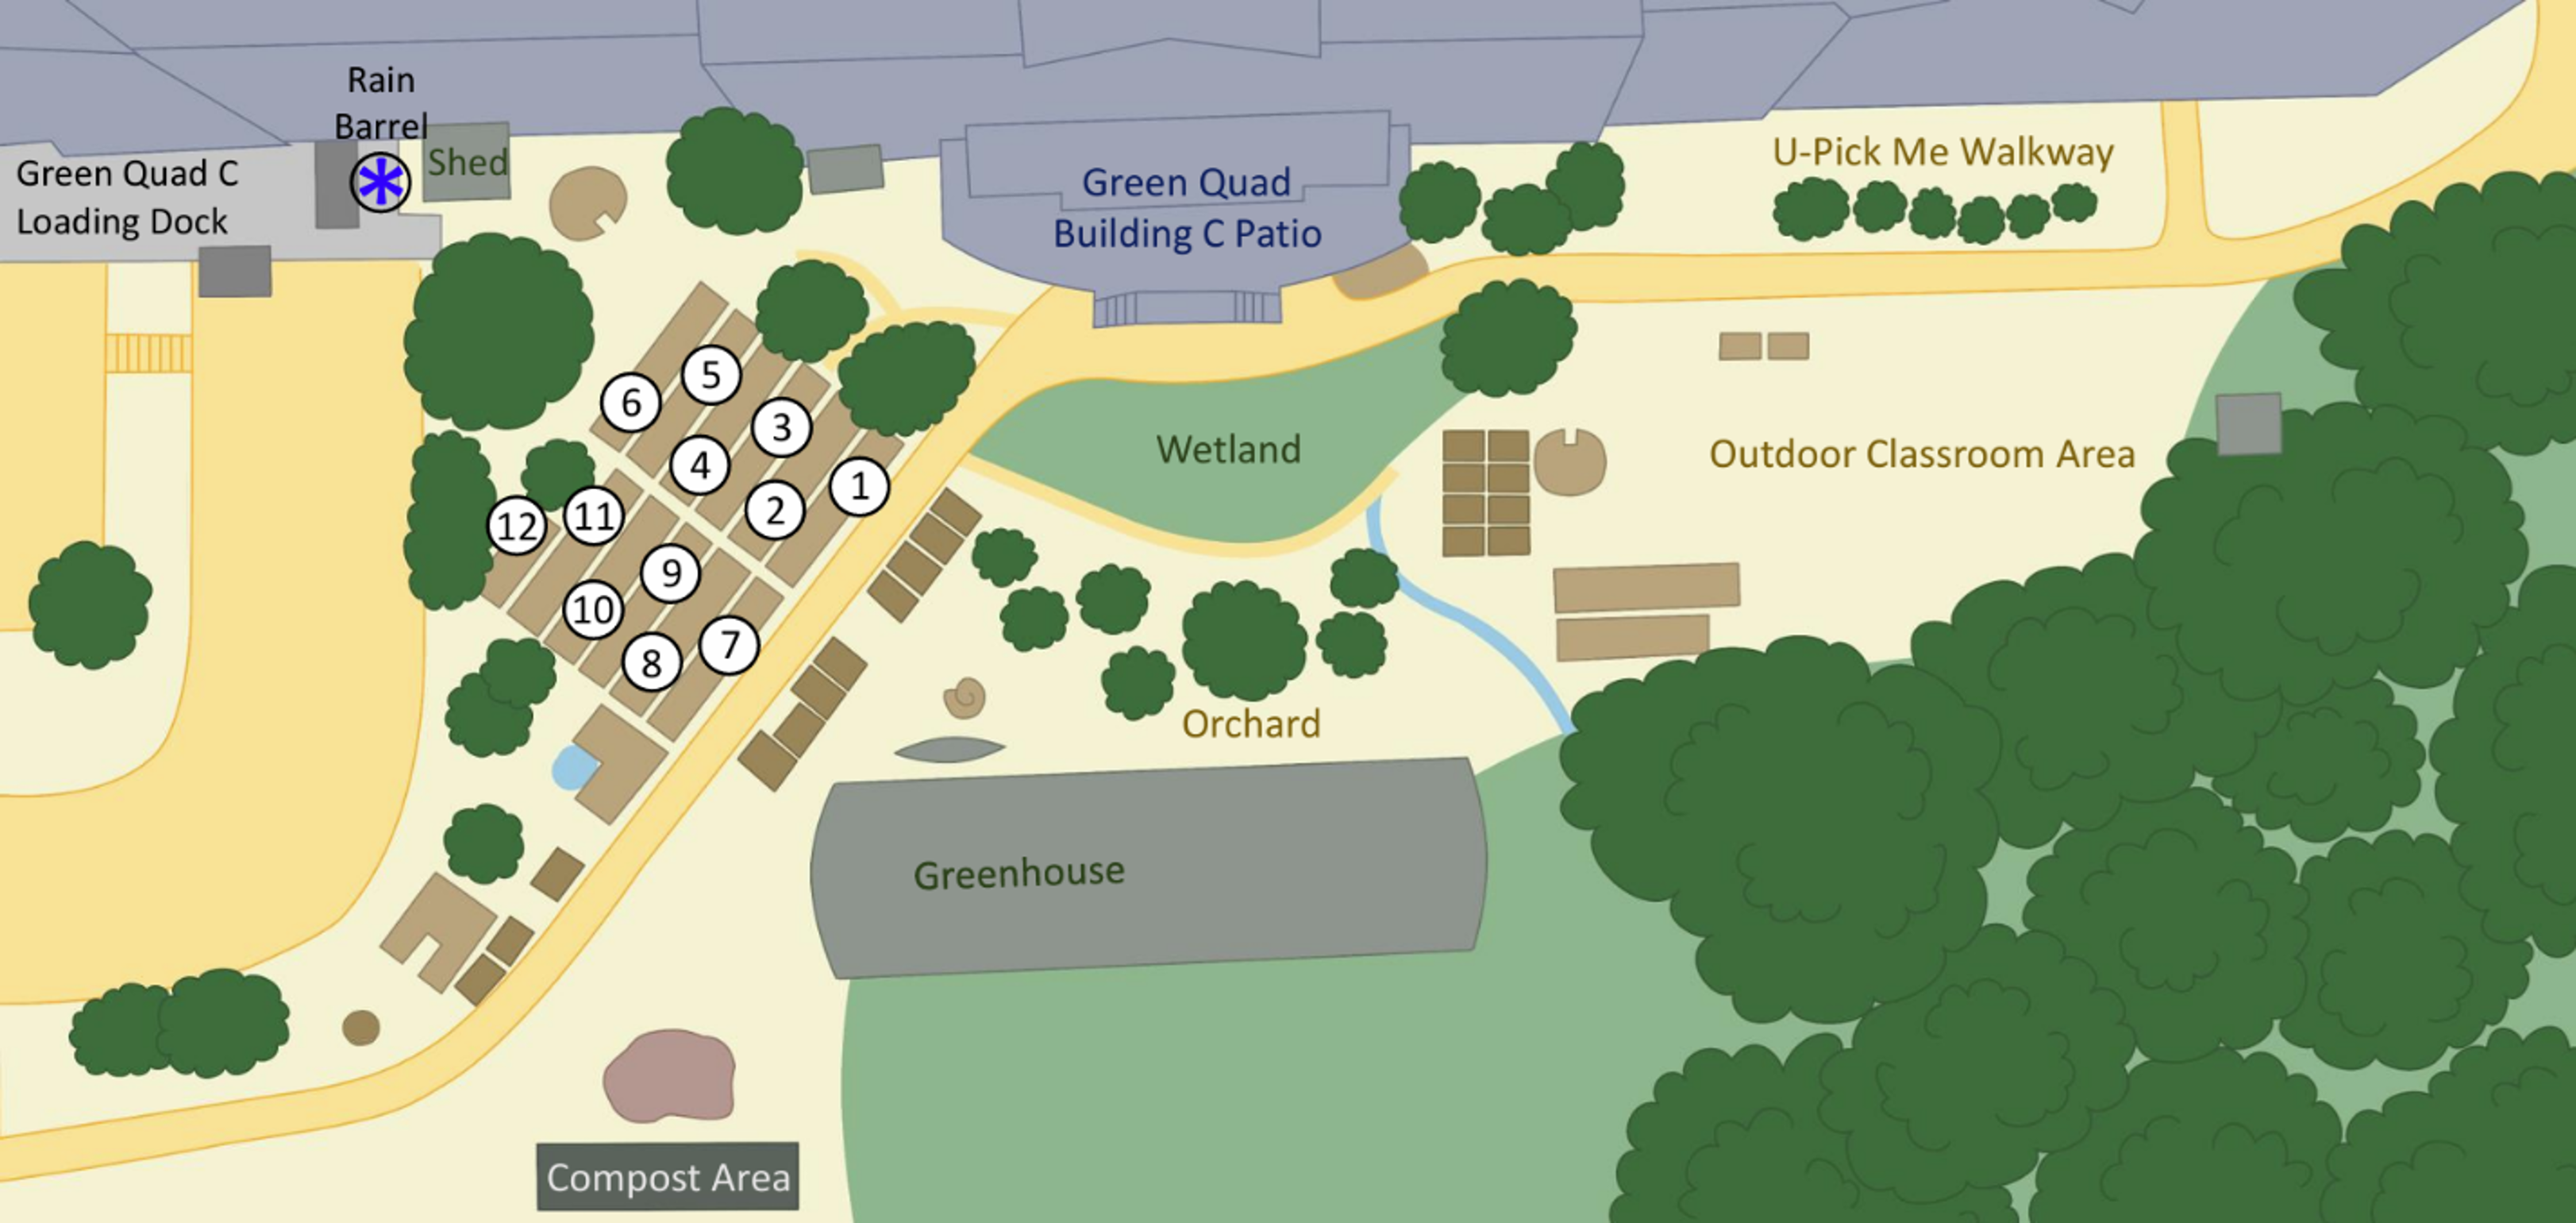
\includegraphics[width=\textwidth]{overview.png}
    \caption{Overview of garden provided by client.}
    \label{fig:overview_garden}
\end{figure}

\begin{figure}[ht]
    \centering
    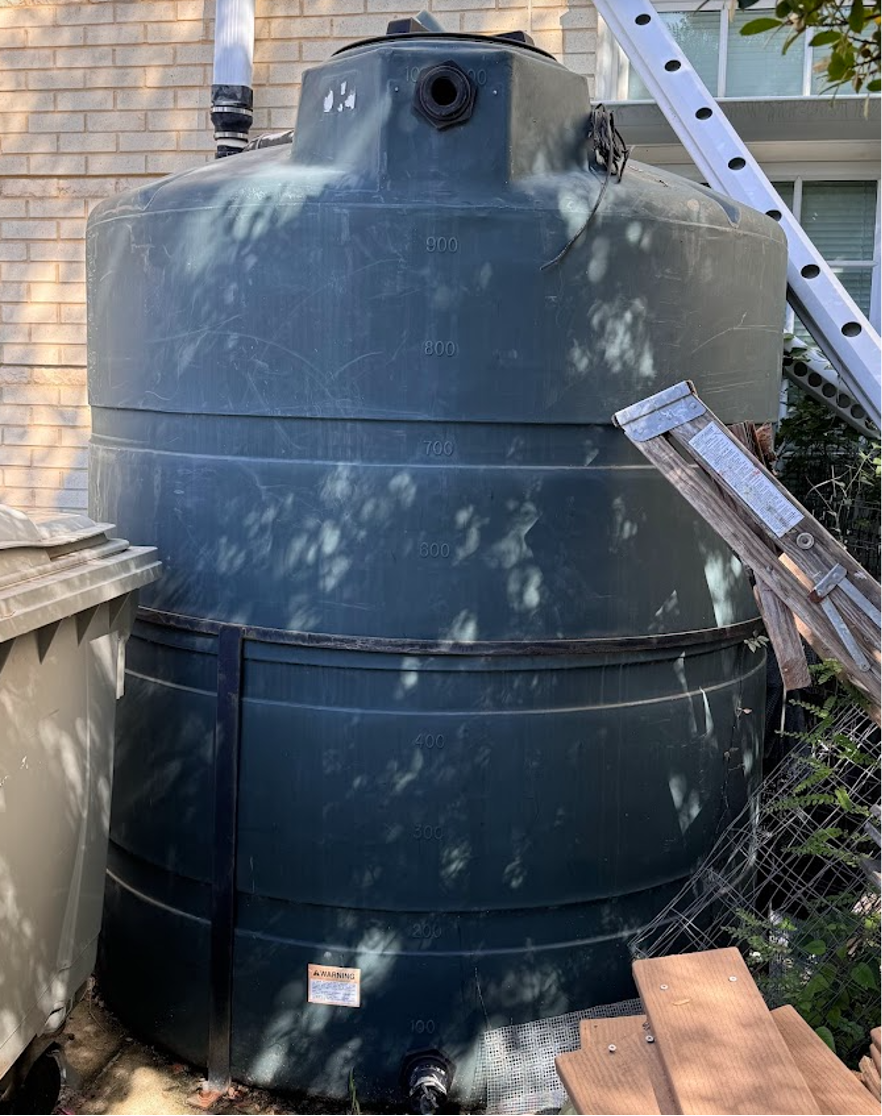
\includegraphics[width=\textwidth]{front.png}
    \caption{Front view of water tank.}
    \label{fig:front_view_tank}
\end{figure}

\begin{figure}[ht]
    \centering
    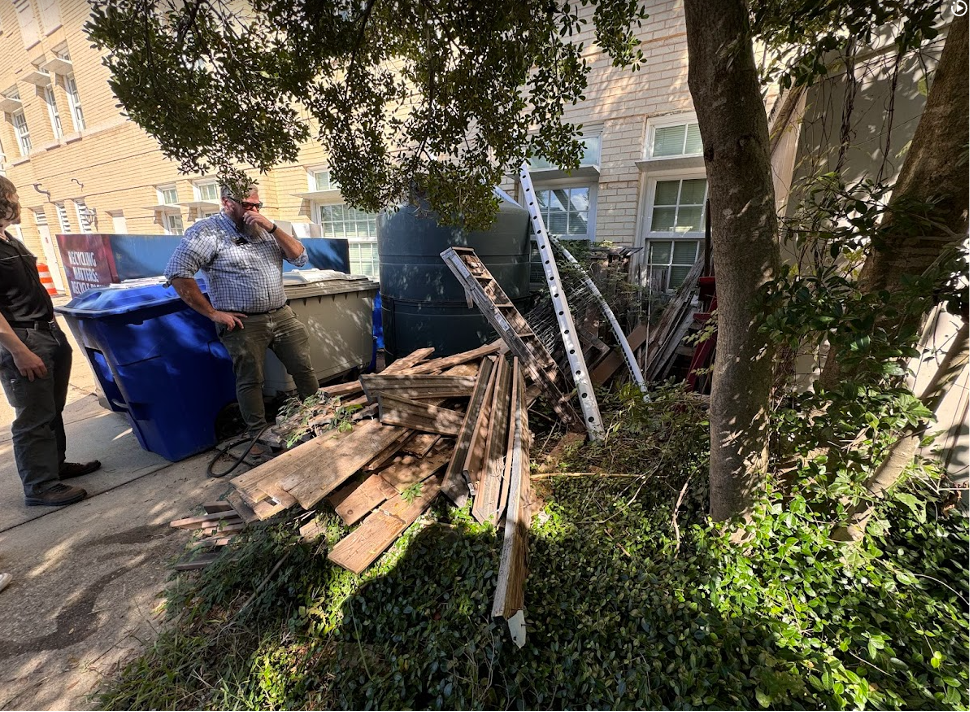
\includegraphics[width=0.7\textwidth]{area.png}
    \caption{View of area surrounding the water tank.}
    \label{fig:area_around_tank}
\end{figure}

\begin{figure}[ht]
    \centering
    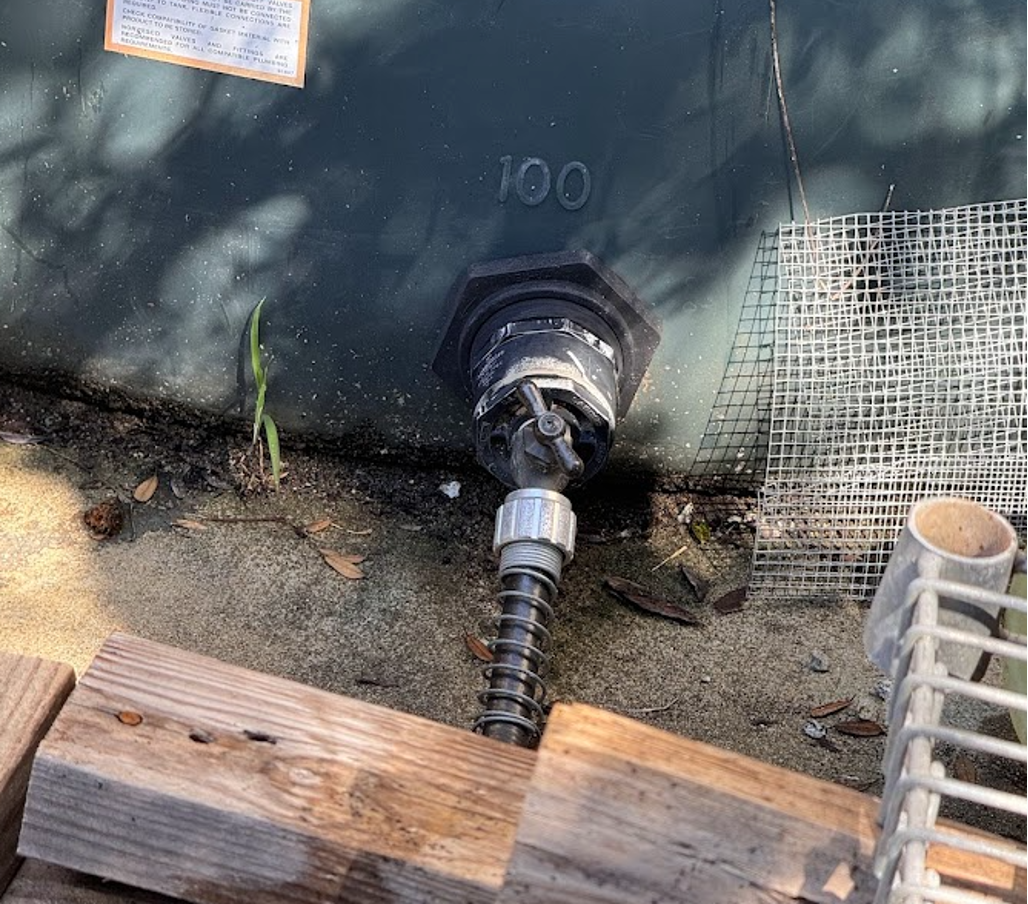
\includegraphics[width=0.7\textwidth]{spigot.png}
    \caption{Spigot for the water tank.}
    \label{fig:spigot_tank}
\end{figure}

\begin{figure}[ht]
    \centering
    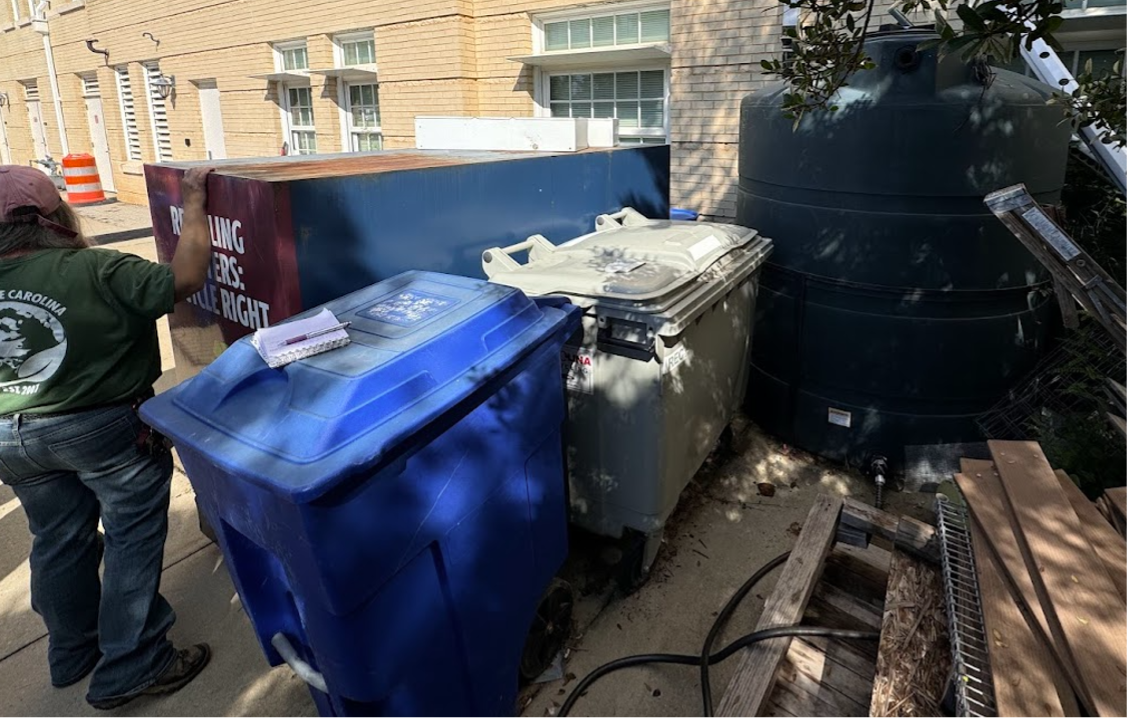
\includegraphics[width=0.9\textwidth]{equipment.png}
    \caption{View of equipment around tank.}
    \label{fig:equipment_around_tank}
\end{figure}

\begin{figure}[ht]
    \centering
    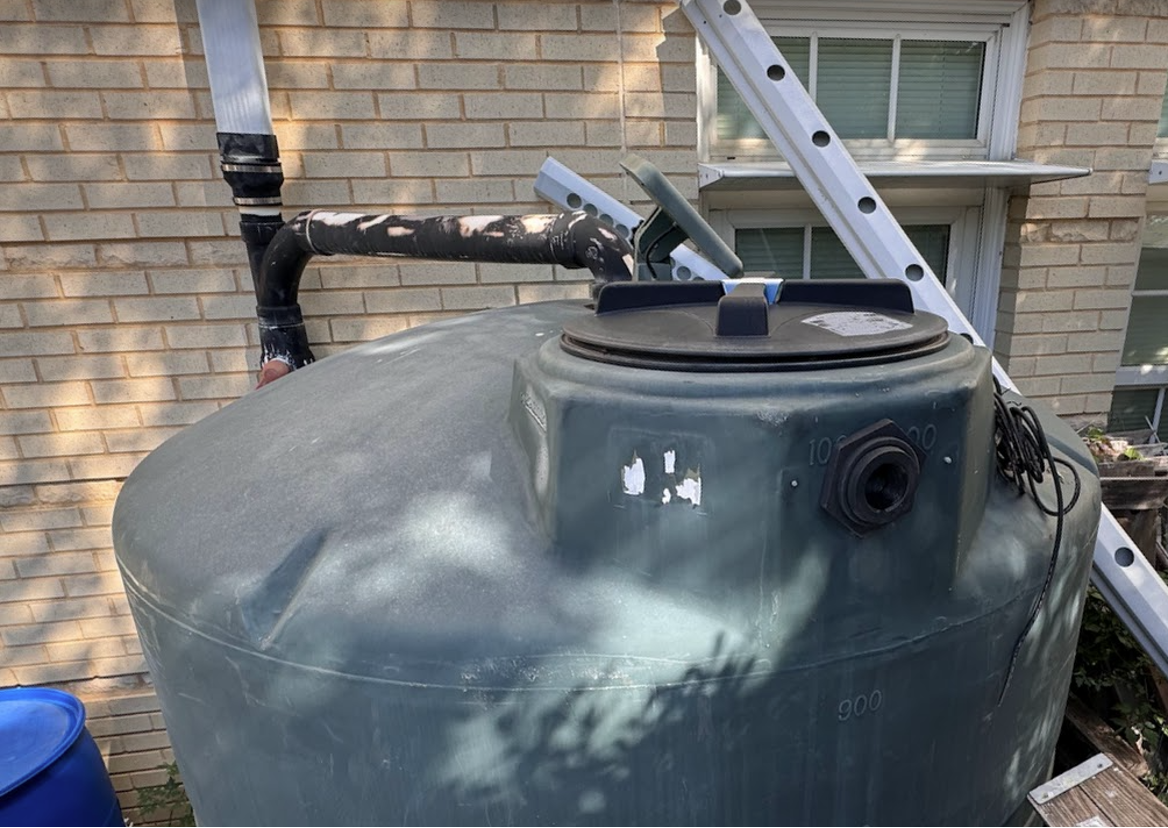
\includegraphics[width=0.8\textwidth]{top.png}
    \caption{Top of tank.}
    \label{fig:top_of_tank}
\end{figure}

\begin{figure}[ht]
    \centering
    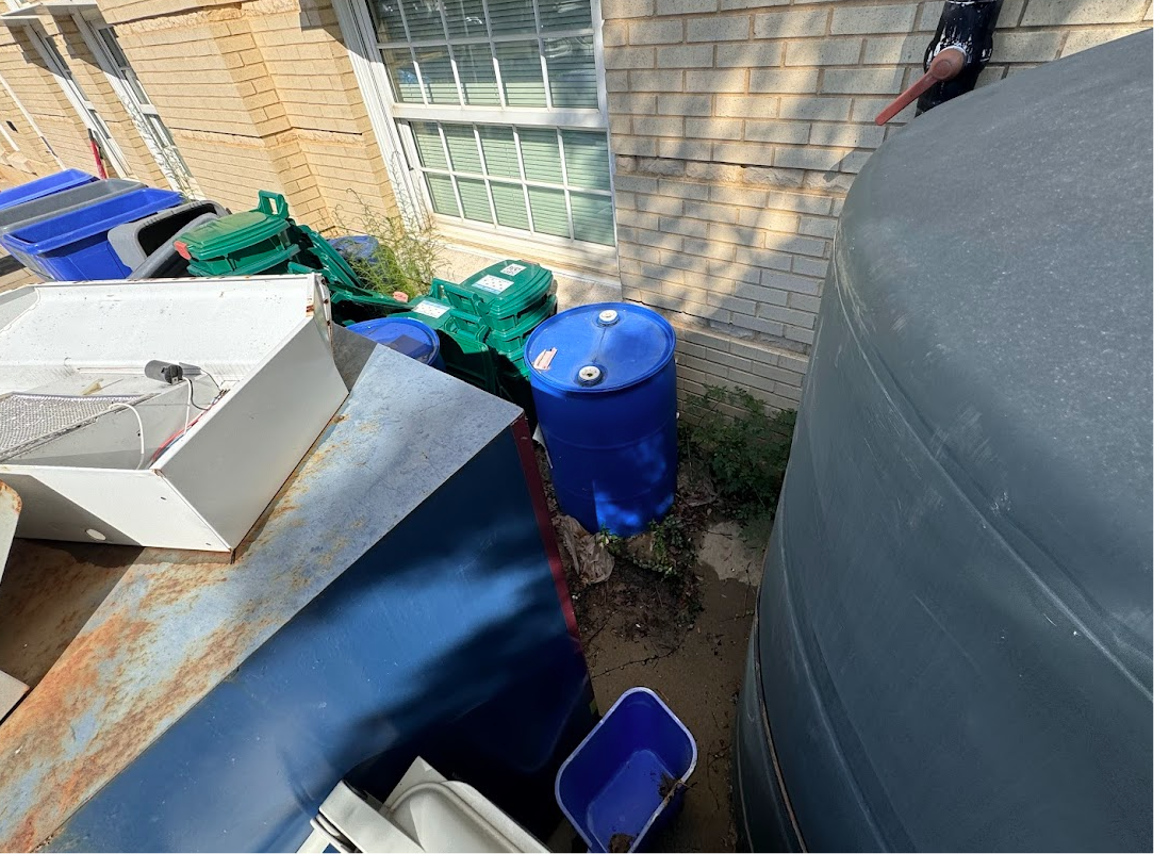
\includegraphics[width=0.7\textwidth]{behind.png}
    \caption{View behind tank.}
    \label{fig:behind_tank}
\end{figure}

\begin{figure}[ht]
    \centering
    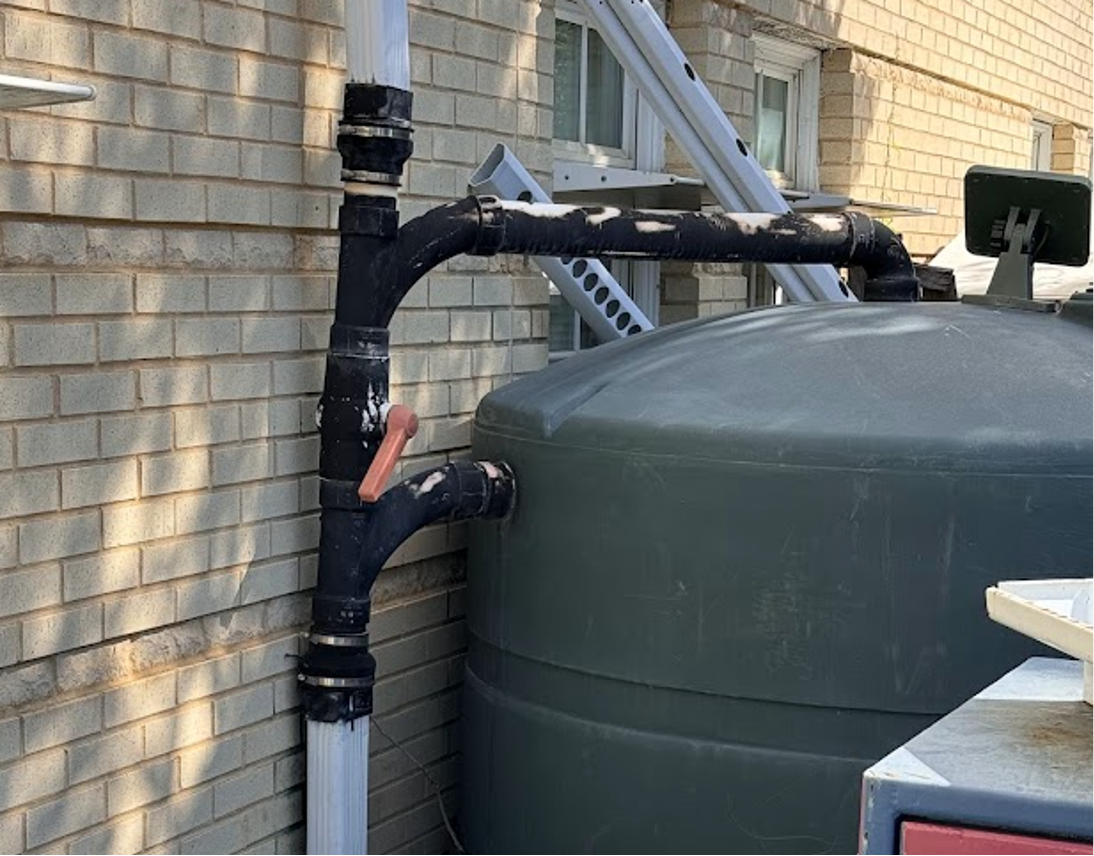
\includegraphics[width=0.7\textwidth]{downspout.png}
    \caption{View of downspout interaction with tank.}
    \label{fig:downspout_interaction}
\end{figure}

\begin{figure}[ht]
    \centering
    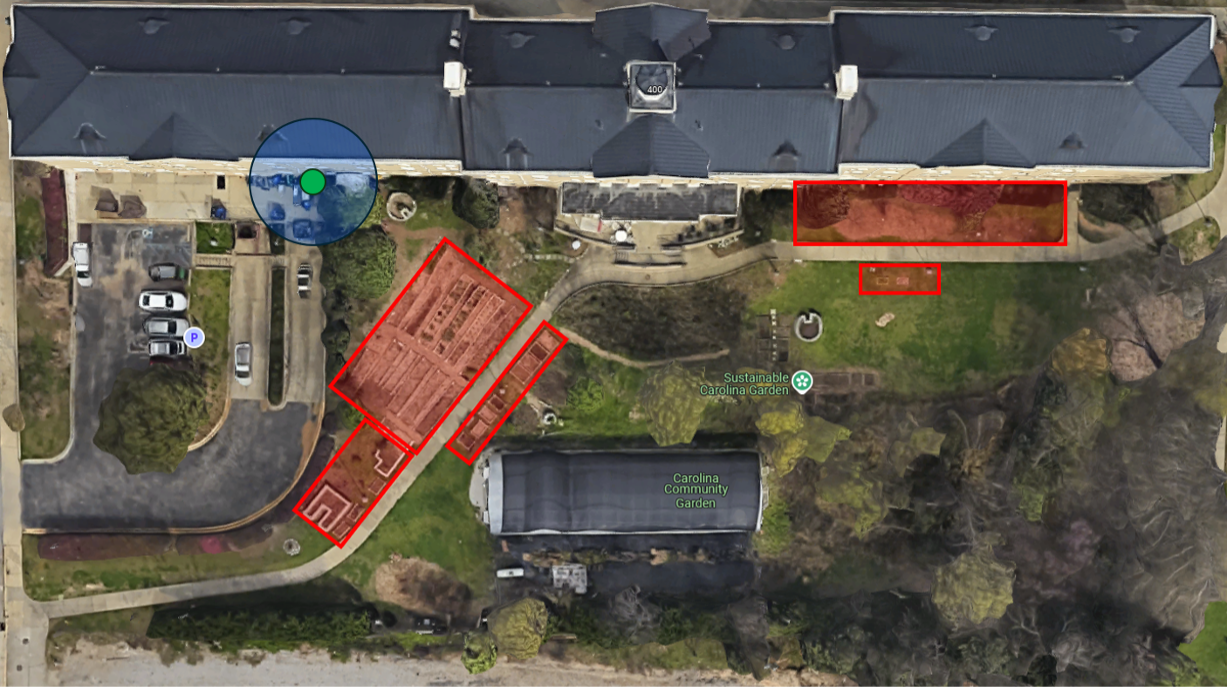
\includegraphics[width=\textwidth]{sat_annotated.png}
    \caption{Satellite view of garden with AOI highlighted.}
    \label{fig:satellite_garden}
\end{figure}

\begin{figure}[ht]
    \centering
    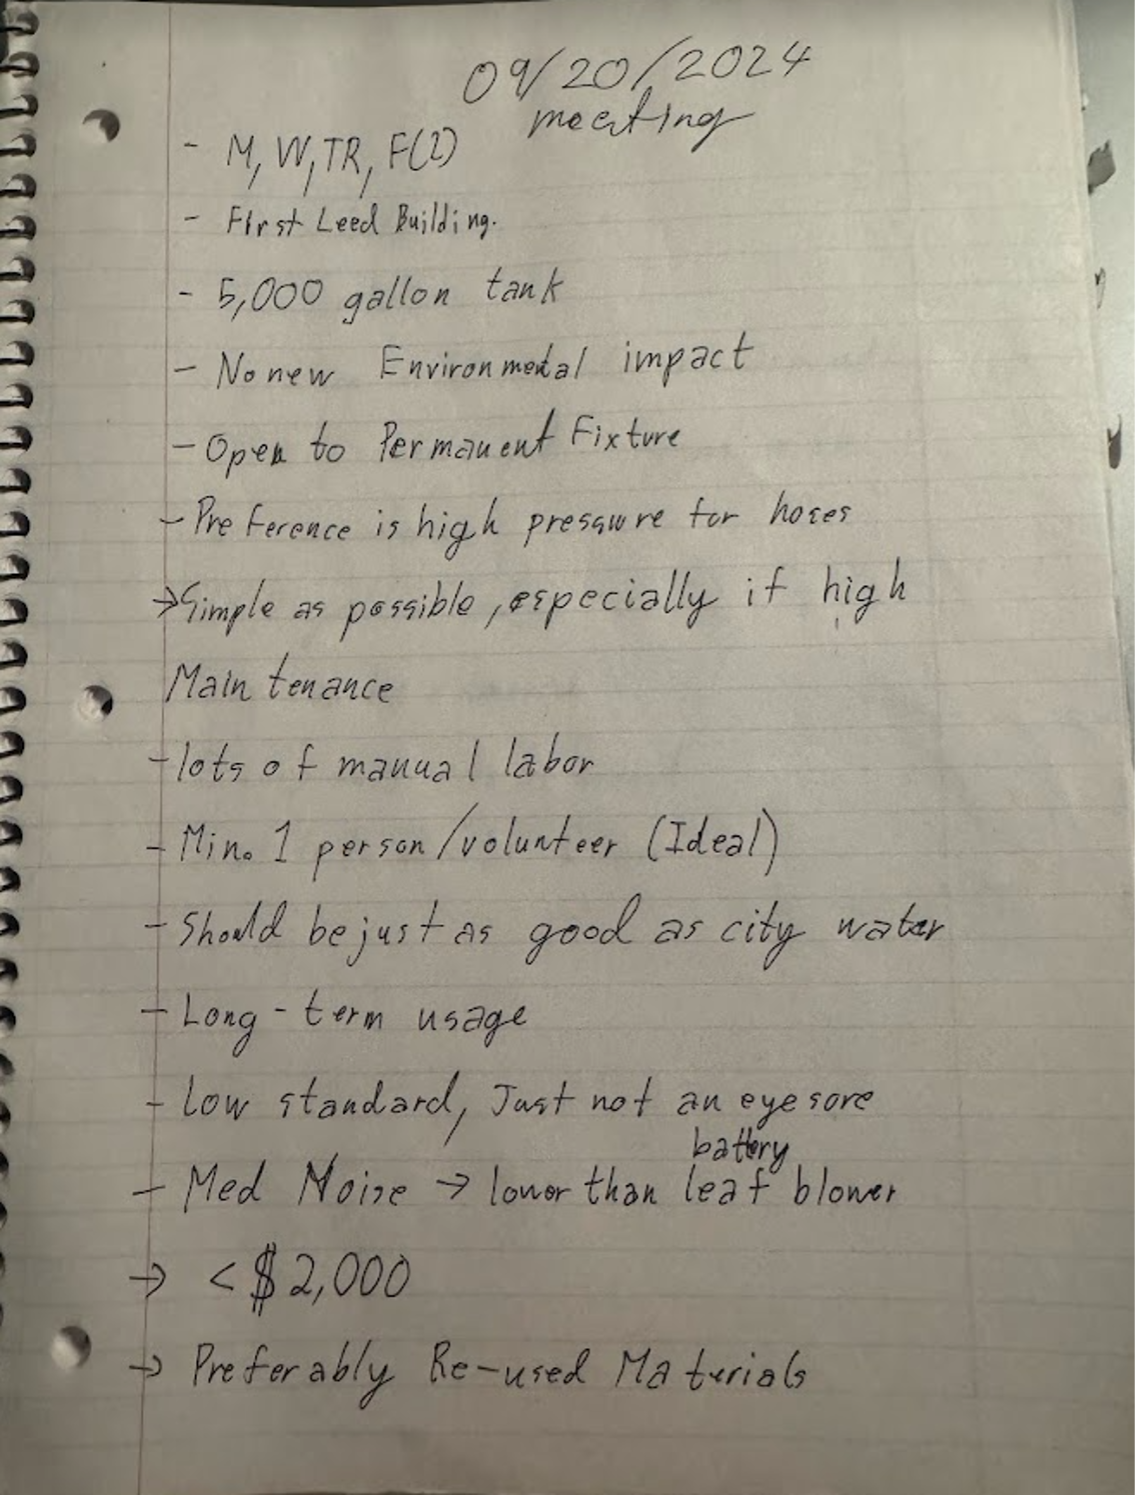
\includegraphics[width=\textwidth]{vaught.png}
    \caption{Notes from meeting J. Vaught.}
    \label{fig:notes_vaught}
\end{figure}

\begin{figure}[ht]
    \centering
    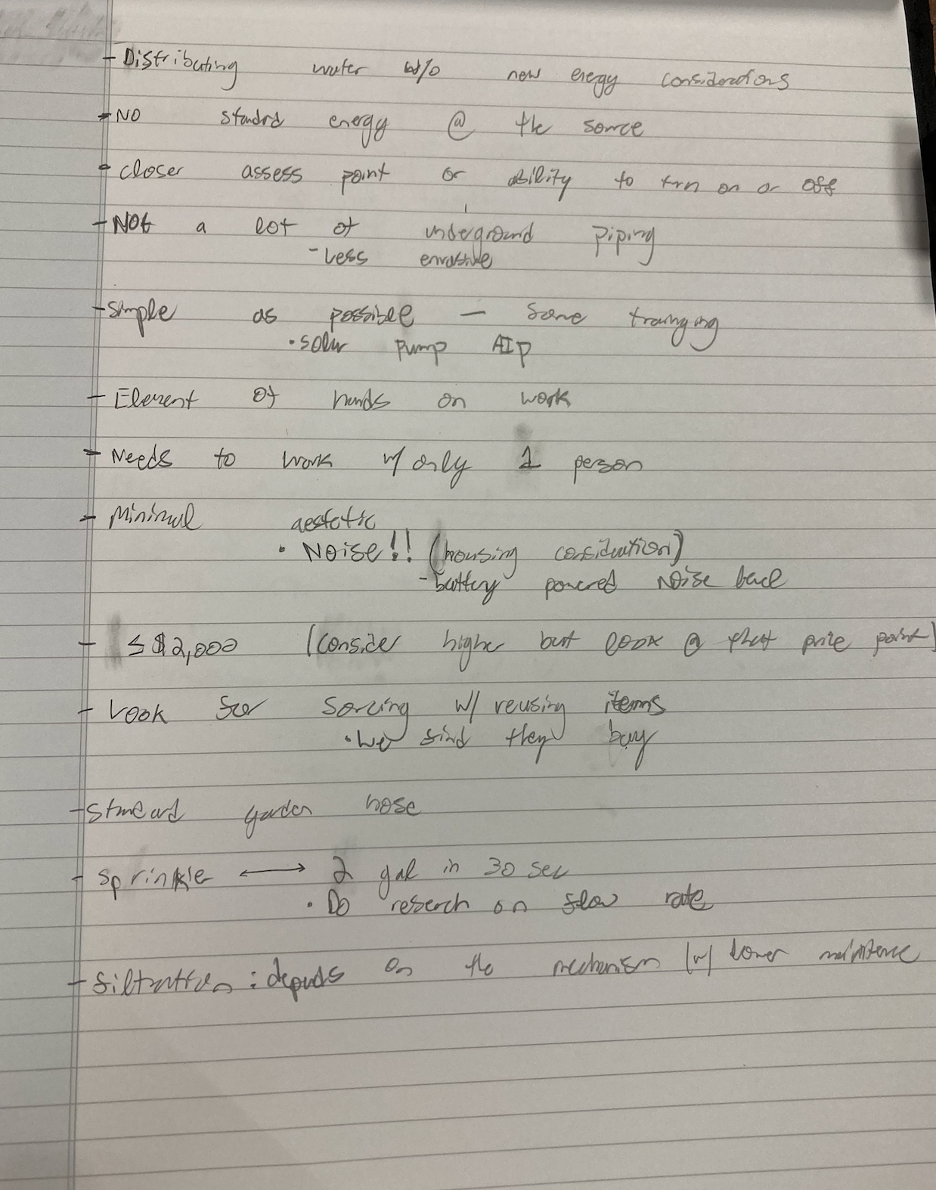
\includegraphics[width=\textwidth]{wenzel.png}
    \caption{Notes from meeting W. Wenzel.}
    \label{fig:notes_vaught}
\end{figure}

\begin{figure}[ht]
    \centering
    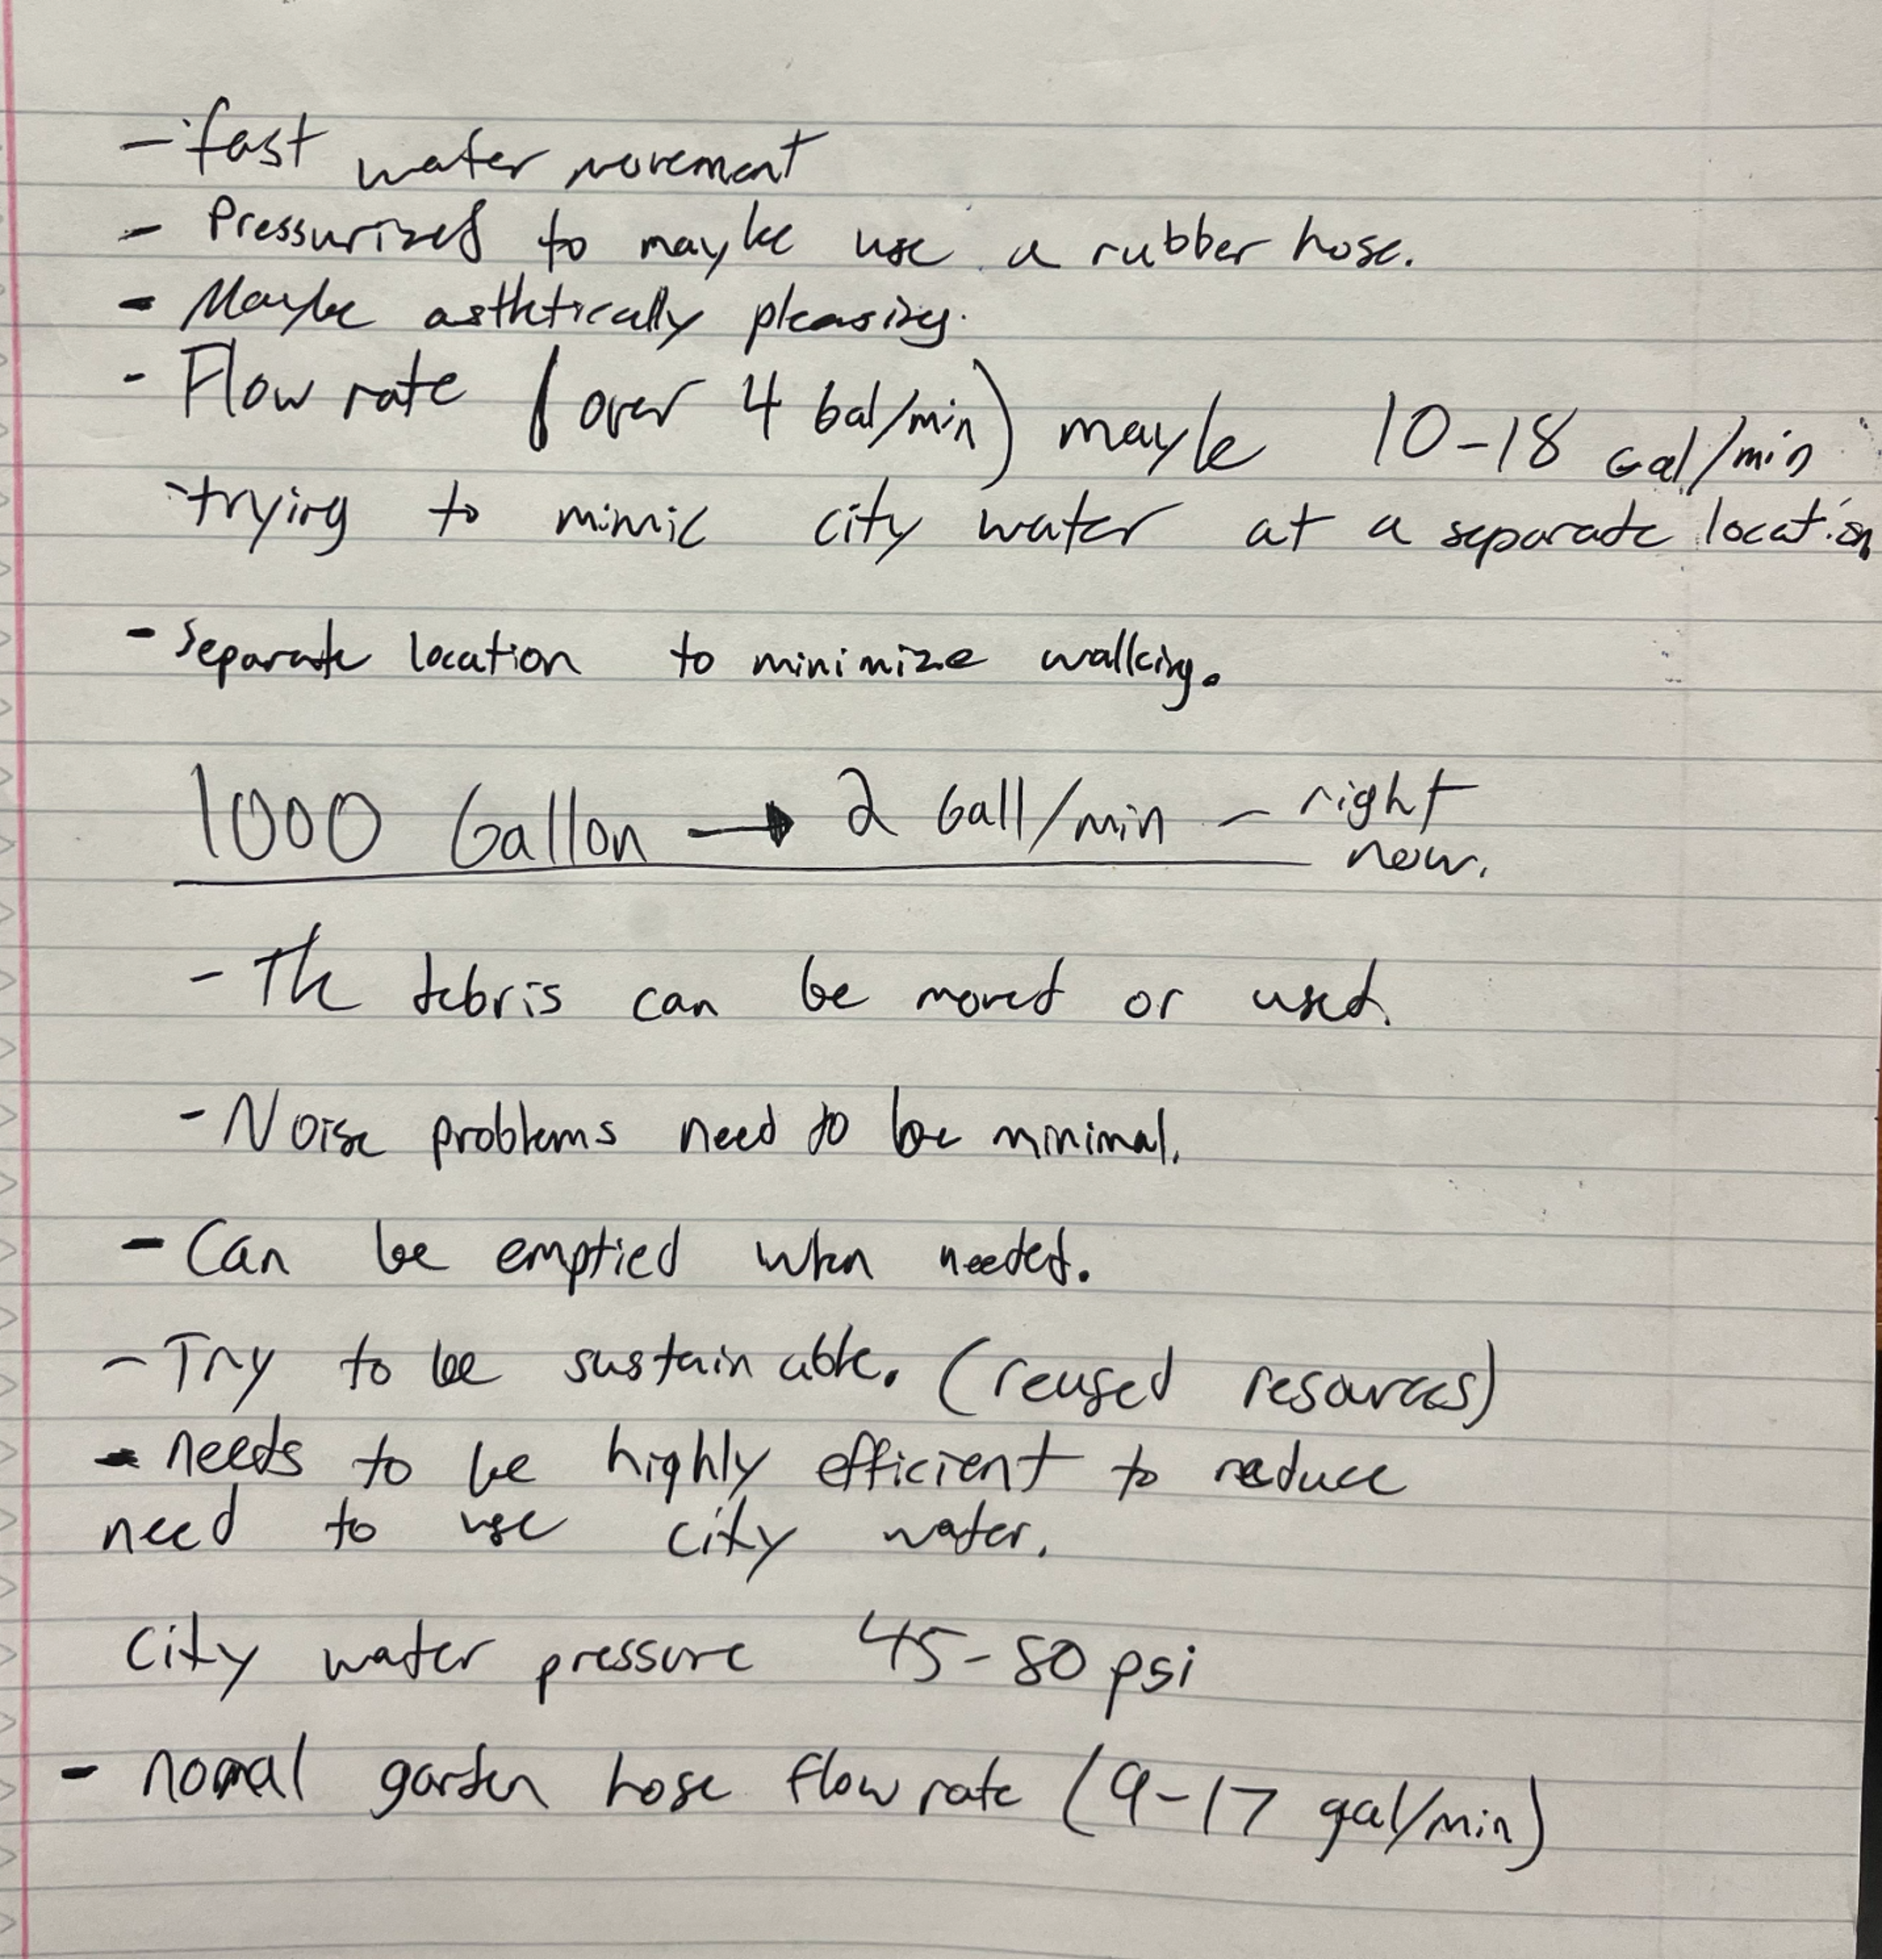
\includegraphics[width=\textwidth]{harmon.png}
    \caption{Notes from meeting T. Harmon.}
    \label{fig:notes_vaught}
\end{figure}

\begin{figure}[ht]
    \centering
    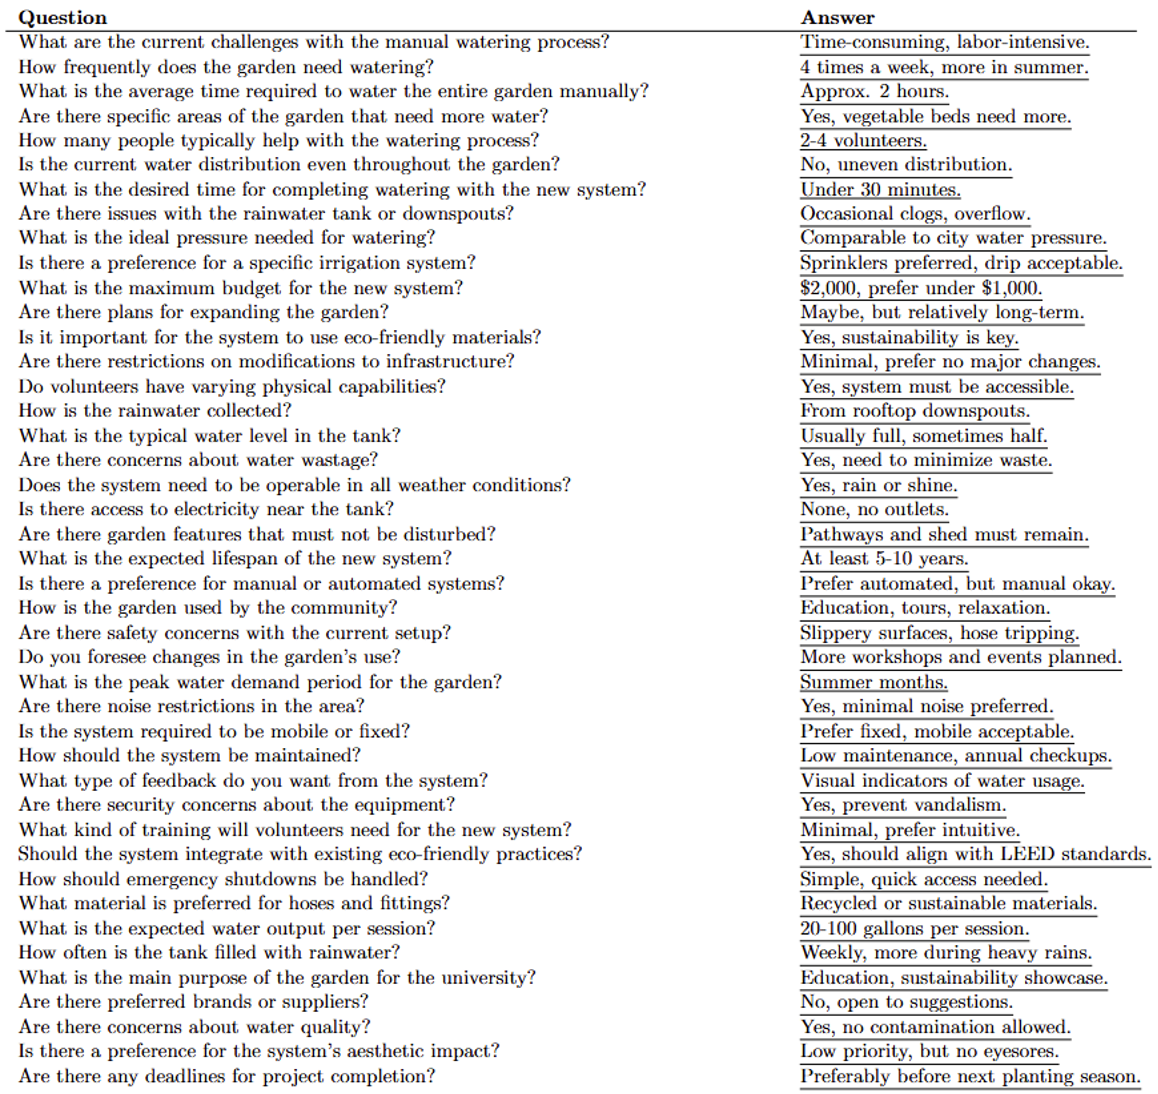
\includegraphics[width=\textwidth]{QA.png}
    \caption{Questions and Answers from meeting with sponsor.}
    \label{fig:qna_sponsor}
\end{figure}







\end{document}